% Trying to break the document up a bit.  This command simply inserts the contents of the file at this point.  It contains the document license, preamble, and title page: things that aren't likely to change more than once.  This can be used to separate discrete parts of a document into files that are easier to edit at one time.
%%%%%%%%%%%%%%%%%%%%%%%%%%%%%%%%%%%%%%%%%%%%%%%%%%%%%%%%%%%%%%%%%%%%%%
% This layout was adapted from one found at latextemplates.com which
% was adapted from another.
%
% License: CC BY-NC-SA 3.0
% (http://creativecommons.org/licenses/by-nc-sa/3.0/)
%
% Original header:
%
% This is a LaTeX version of the sample laboratory report from
% Virginia Tech's copyrighted 08-09 CHEM 1045/1046 lab manual.
% Reproduction of this one appendix section for academic purposes
% should fall under fair use.
%
%%%%%%%%%%%%%%%%%%%%%%%%%%%%%%%%%%%%%%%%%%%%%%%%%%%%%%%%%%%%%%%%%%%%%%

\documentclass{article}

\usepackage{graphicx}
% \usepackage[acronym]{glossaries} % Lets us use acronyms
\usepackage{multicol}
\usepackage{amsmath}
\usepackage{siunitx} % SI units in math mode
\usepackage{subcaption}

\author{}
\title{ELEC-313 \\ Lab 5: CMOS Circuits\\ }
\date{\today}

% \loadglsentries{acronyms} % Actually loads 'acronyms.tex'
% \makeglossaries

\begin{document}

\maketitle

\begin{center}
  \begin{tabular}{lr}
    Date Performed: & October 16, 2013 \\
    Partners:       & Charles Pittman    \\
    & Stephen Wilson     \\
  \end{tabular}
\end{center}

\newpage

\tableofcontents
\listoffigures
\listoftables
\newpage

% Number the enumerate environment (unordered lists) by letter:
\renewcommand{\labelenumi}{\alph{enumi}.}

\section{Objective}
\label{sec:objective}


\section{Equipment}
\label{sec:equipment}

\begin{tabular}{ll}
  \centering
  Transistor: 2N7000               & Power supply: HP E3631A            \\
  Function Generator: HP 33120 & Multimeter: HP 34401A              \\
  Oscilloscope: Agilent 54622D & Capacitors: \SI{0.1}{\micro\farad} \\
  \multicolumn{2}{l}{Resistors: \SI{100}{\ohm}, \SI{300}{\ohm}, \SI{470}{\ohm}, \SI{1}{\kilo\ohm} (x2) \SI{33}{\kilo\ohm}, \SI{100}{\kilo\ohm} (x2)} \\
\end{tabular}

\section{Schematics}
\label{sec:schematics}

% \begin{figure}[hbtp]
%   \centering
%   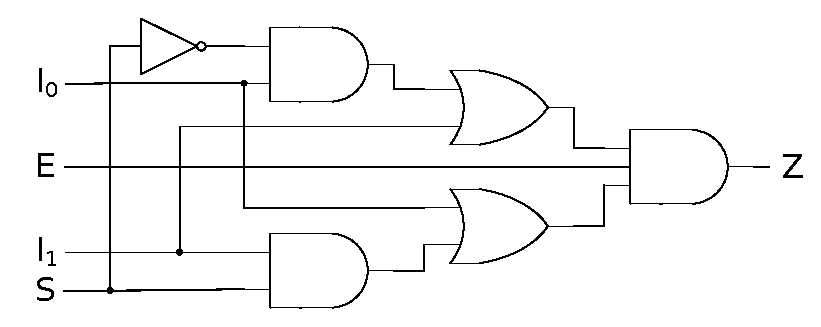
\includegraphics[width=0.6\textwidth]{circuit}
%   \caption{\label{fig:circuit} Circuit used in this lab.}
% \end{figure}

\begin{figure}[hbtp]
  \centering
  \begin{subfigure}[b]{0.4\textwidth}
    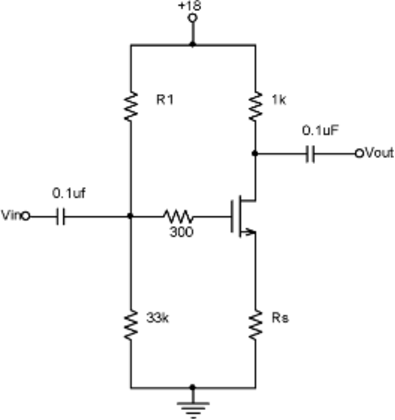
\includegraphics[width=\textwidth]{common-source}
    \caption{\label{schem:common-source} Common-source amplifier}
  \end{subfigure}%
  ~
  \begin{subfigure}[b]{0.4\textwidth}
    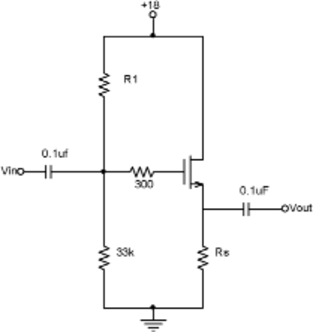
\includegraphics[width=\textwidth]{source-follower}
    \caption{\label{schem:source-follower} Source-follower amplifier}
  \end{subfigure}
  \caption{\label{fig:schematics} Circuits used in this lab. $R_1=\SI{100}{\kilo\ohm}$,  $R_s=\SI{470}{\ohm}$}
\end{figure}

\section{Procedure}
\label{sec:procedure}

\subsection{Common-Source Amplifier}

\subsection{Source-Follower Amplifier}

\section{Results}

\subsection{Common-Source Amplifier}

\begin{table}[hbtp]
  \centering
  \begin{tabular}{cccc}
    $V_G$ & $V_D$ & $V_S$ & $I_D$ \\
    \hline
    \SI{4.391}{V} & \SI{13.498}{V} & \SI{2.11}{V} & \SI{4.52}{mA} \\
  \end{tabular}
  \caption{\label{tab:tran_common} Transistor characteristics}
\end{table}

\begin{table}[hbtp]
  \centering
  \begin{tabular}{cc}
    $V_{in}$ (\si{mV}) & $V_{out}$ (\si{V}) \\
    \hline
    200          & 0.382         \\
    300          & 0.566         \\
    400          & 0.760         \\
    500          & 0.939         \\
    600          & 1.140         \\
    700          & 1.340         \\
    800          & 1.530         \\
    900          & 1.721         \\
    1000         & 1.90          \\
  \end{tabular}
  \caption{\label{tab:common-source} Common-source amplifier}
\end{table}

\subsection{Source-Follower Amplifier}

\begin{table}[hbtp]
  \centering
  \begin{tabular}{cccc}
    $V_G$ & $V_D$ & $V_S$ & $I_D$ \\
    \hline
    \SI{4.391}{V} & \SI{18.003}{V} & \SI{2.12}{V} & \SI{4.579}{mA} \\
  \end{tabular}
  \caption{\label{tab:tran_follower} Transistor characteristics}
\end{table}

\begin{table}[hbtp]
  \centering
  \begin{tabular}{cc}
    $V_{in}$ (\si{mV}) & $V_{out}$ (\si{mV}) \\
    \hline
    200                & 182                 \\
    300                & 268                 \\
    400                & 360                 \\
    500                & 451                 \\
    600                & 541                 \\
    700                & 634                 \\
    800                & 725                 \\
    900                & 813                 \\
    1000               & 906                 \\
  \end{tabular}
  \caption{\label{tab:source-follower} Source-follower amplifier}
\end{table}

% \begin{table}[hbtp]
%   \centering
%   \begin{tabular}{c|ccc}
%     $V_{TN}$ = \SI{2.11}{V} & $V_{DS}$ = \SI{0.5}{V} & $V_{DS}$ = \SI{1}{V} & $V_{DS}$ = \SI{1.5}{V} \\
%     \hline
%     $V_{GS}$ = \SI{2.91}{V} & & & 0.1078 \\
%     $V_{GS}$ = \SI{2.71}{V} & & 0.0931 & \\
%     $V_{GS}$ = \SI{2.51}{V} & 0.07688 & & \\
%   \end{tabular}
%   \caption{\label{tab:kn} $k_n'$}
% \end{table}

% \begin{figure}[hbtp]
%   \centering
%   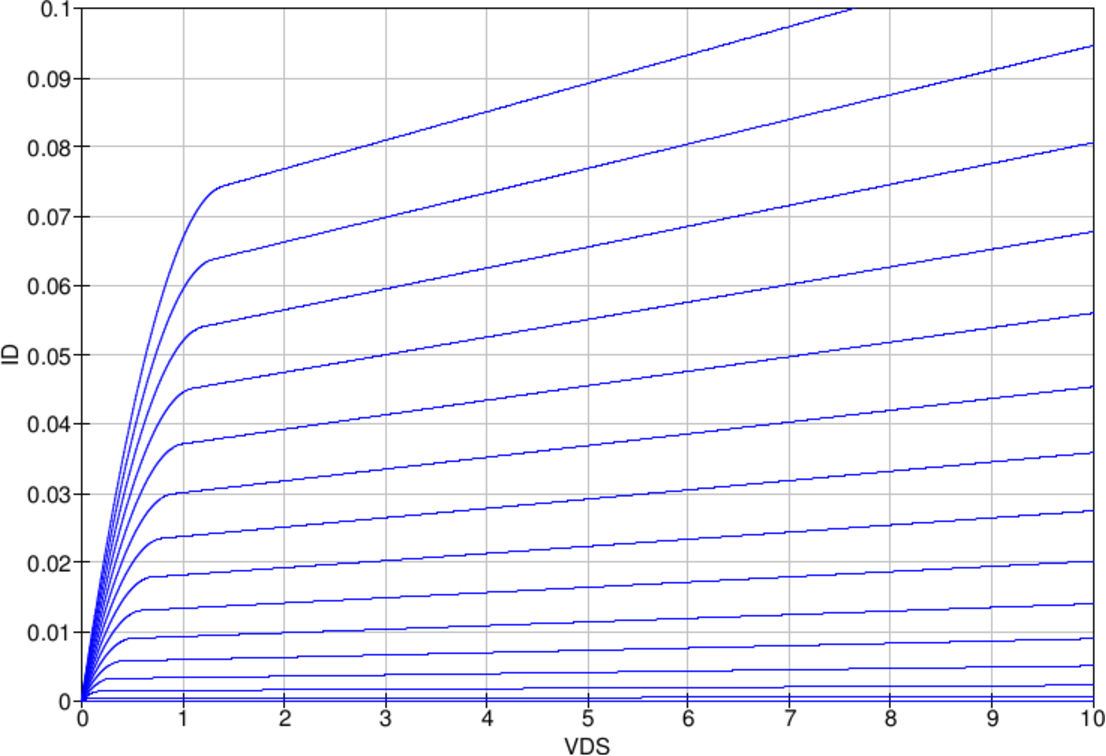
\includegraphics[width=0.9\textwidth]{lambda6}
%   \caption{\label{fig:lambda6} PSpice Simulation. $\lambda$ = 0.06}
% \end{figure}

\section{Conclusion}
\label{sec:conclusion}


\section{Equations}
\label{sec:equations}

% LaTeX sees blank lines as a start of another paragraph.  To avoid
% unnecessary vertical spaces between equations, and still visually
% separate in source, put a comment between them.
%
\begin{equation}
  \label{eq:amp}
  V_{o,L} = V_{o,NL} \frac{R_L}{R_o + R_L}
\end{equation}
%
% \begin{equation}
%   \label{eq:phys}
%   \frac{k_n'}{2} \cdot \frac{W}{L} = \frac{I_{D1}}{(V_{GS1} - V_{TN})^2}
% \end{equation}

\end{document}
